\documentclass{article}
\usepackage[utf8]{inputenc}
\usepackage{vmargin}

\setpapersize{A4}
\setmargins{2.5cm}  % MARGEN IZQ.
{1.5cm}             % MARGEN SUPERIOR
{16.5cm}            % ANCHO DEL TEXTO
{23.42cm}           % ALTURA TEXTO
{10pt}              % ALTURA ENCABEZADOS
{1cm}               % ESPACIO ENTRE TEXTO Y ENCABEZADOS
{0pt}               % ALTURA DE PIE Y PÁGINA
{2cm}               % ESPACIO TEXTO Y PIE DE PÁGINA



 %% FUENTES DEL DOCUMENTO %%

\font\titulo=cmr12 at 40pt
\font\cuerpo=cmr12 at 13pt

\usepackage{natbib}
\usepackage{graphicx}

%% EMPIEZA DOCUMENTO %%%%%
\begin{document}

    \begin{titlepage}
        \centering
        {\bfseries\LARGE Universidad de Almería\par}
        \vspace{1cm}
        {\scshape\Large Escuela Superior de Ingeniería - Ingeniería Informática \par}
        \vspace{1cm}
        {\scshape\Huge Como elaborar una buena memoria - Problema NRP 2\par}
        \vspace{2cm}
        {\itshape\LARGE Procesos de Ingeniería del Software 2 \par}
            \begin{figure}[h!]
            \centering
            
\includegraphics[scale=0.85]{ESI}
            \end{figure}
            {\Large 25 de Febrero de 2021 \par}
        \vspace{2cm}
            {\Large Autores: \par}
            {\Large Pablo Almansa Torress \par}
            {\Large Daniel Ortega Rubio \par}
            {\Large Juan José Pallarés Sánchez \par}
            {\Large Pablo Daniel Estévez Bretones \par}
        \vspace{2cm}
    
    \end{titlepage} 

\section{Funciones en LateX}
\cuerpo En esta sección lo que haremos será comentar paso a paso como hemos implementado la función según se nos cuenta en el enunuciado.\\


Lo primero que hemos hecho ha sido es crear el elemento flotante, esto lo haremos creando una función llamada \textbf{''newfloat''} que tendrá tres parámetros. El primero de los tres parametros define el objeto. El primer parámetro es el nombre del objeto, la segunda es la numeración que usaremos para ese tipo de objeto y la tercera es el texto del subtitulo que llevará el objeto.\\\\


\begin{figure}[h!]
\centering
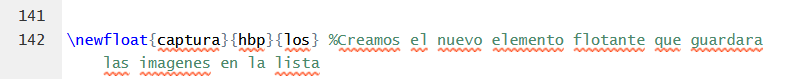
\includegraphics[scale=1]{CAP1}
\caption{Función newfloat}
\label{fig:cap1}
\end{figure}

En la siguiente linea tenemos que dar un nombre a la imagen que aparecerá cada vez que insertemos una, y que irá junto con su número. \\


\begin{figure}[h!]
\centering
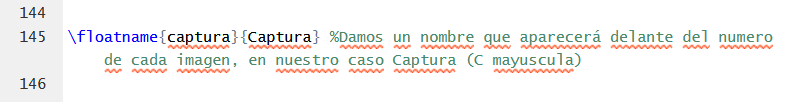
\includegraphics[scale=1]{CAP2}
\caption{Función floatname}
\label{fig:cap1}
\end{figure}

Ahora lo que tenemos que hacer es crear el comando para insertar la lista de capturas que se nos pide en el enunciado. Para ello usamos los comandos \textbf{''listofcapturas''}, que será el comando al que llamaremos, además de \textbf{''listof''}, que nos servirá para hacer una lista de capturas (primer parámetro) llamada \textbf{''Lista de capturas''} (segundo parámetro) \\\\\\\\\

\begin{figure}[h!]
\centering
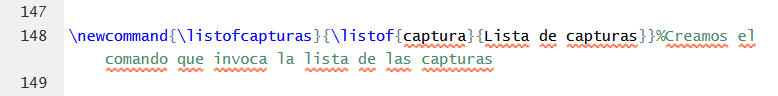
\includegraphics[scale=1]{CAP3}
\caption{Creacion función listofcapturas}
\label{fig:cap1}
\end{figure}

Después, vamos a crear el comando para insertar los 3 parametros y utilizar las funciones citadas anteriormente. Lo primero que hacemos en este nuevo comando es llamar al objeto captura. Luego centramos la imagen y el subtitulo que vamos a añadir, que es la linea 158. Además de que en la siguiente linea etiquetamos estas imágenes.\\

\begin{figure}[h!]
\centering
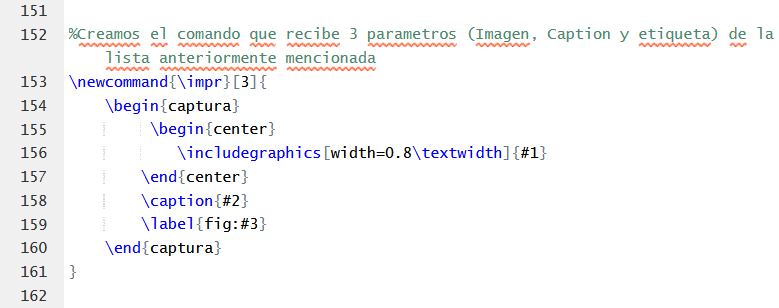
\includegraphics[scale=1]{CAP4}
\caption{Comando "impr"}
\label{fig:cap1}
\end{figure}

Y por último y más importante, vamos a comprobar que funciona. Primero insertamos la ultima función que hemos descrito, para ello en el documento ''contenido2.tex'' insertamos los comandos con sus parámetros: el nombre del archivo y su etiqueta: \\ 

\begin{figure}[h!]
\centering

\includegraphics[scale=1]{PRUEBA1.PNG}
\caption{LLamada a la función "impr"}
\label{fig:cap1}
\end{figure}

Ahora vemos en el documento si las capturas se encuentran y tienen los requisitos que se nos pide, es decir, están en una lista aparte donde su enumeración es, por tanto, independiente del resto de figuras: \\

\begin{figure}[h!]
\centering
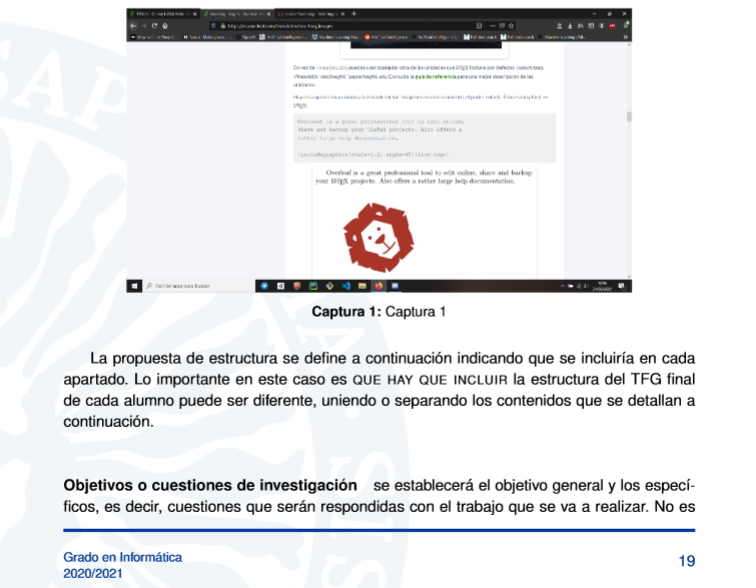
\includegraphics[scale=0.57]{PRUEBA2.PNG}
\caption{LLamada a la función "impr", primera captura}
\label{fig:cap1}
\end{figure}

\begin{figure}[h!]
\centering
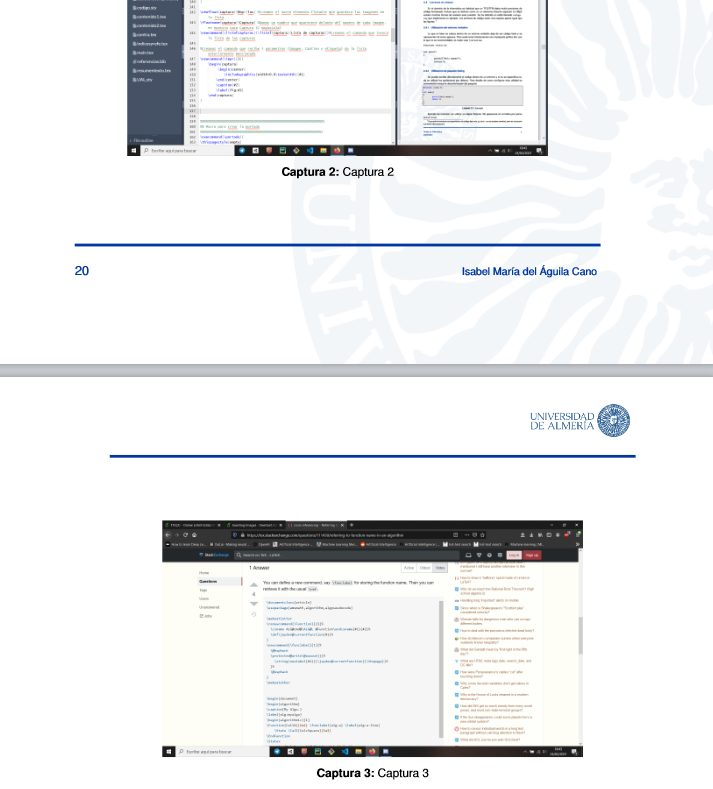
\includegraphics[scale=0.65]{PRUEBA3.PNG}
\caption{LLamada a la función "impr", segunda y tercera captura}
\label{fig:cap1}
\end{figure}


%% ESPACIO ENTRE SECCIONES %%%%%%%%%%%%%%%%%%
\vspace{1cm}


%% NUEVA SECCIÓN %%%%%%%%%%%%%%%%%%%

\section{Organización dentro del proyecto. Issues en github}
\cuerpo En esta sección explicaremos como nos hemos organiado para realizar la práctica.\\

    \begin{itemize}
      
    	\item Github: La persona que se ha encargado principalmente de la creación de issues en el proyecto de Github ha sido Juan José. Él ha creado las issues, las ha asignado a los miembros del equipo y las ha cerrado cuando se han terminado. Aqui se pueden ver las tareas realizadas y las que quedan por hacer, respectivamente:\\\\
    	
    	\begin{figure}[h!]
        \centering
        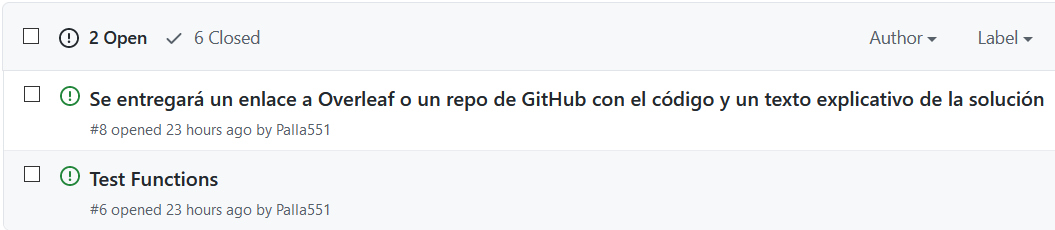
\includegraphics[scale=0.65]{GIT1.PNG}
        \label{fig:cap1}
        \end{figure}
        
        \begin{figure}[h!]
        \centering
        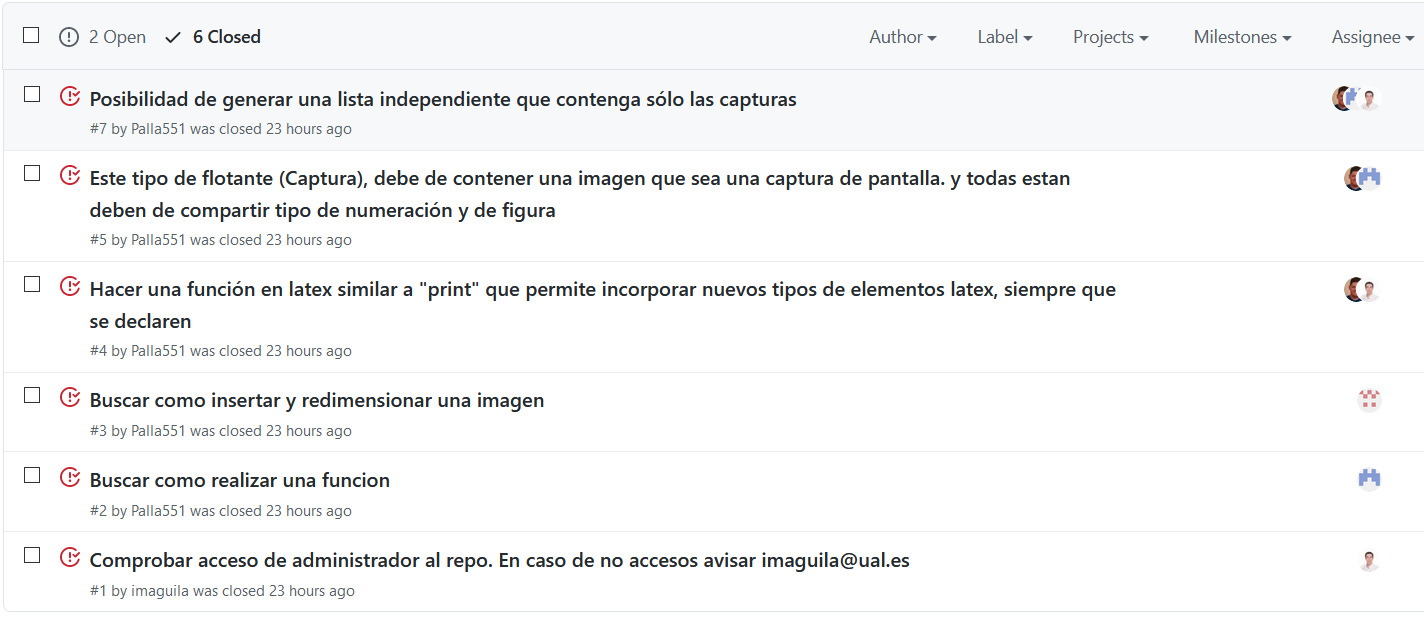
\includegraphics[scale=0.55]{GIT2.PNG}
        \label{fig:cap1}
        \end{figure}

        \vspace{1.95cm}
    
    	\item Desarrollo de la función: Principalmente, las personas que han desarrollado la función en Latex han sido Daniel, Pablo y Juan José. La función se ha ido desarrollando consultado frecuentemente la documentación oficial de Latex y probando cada vez que se hacia algun cambio cual era el resultado de este. Como también se puede observar en las capturas de la sección anterior, se han comentado las lineas de documento latex que se han ido haciendo para dejar constancia de funcionalidad tanto a la profesora como a cualquiera de nosotros que necesite buscar algo similar en el futuro.\\
    
    	\item Prueba: A la hora de probarlo, ha sido Pablo Daniel junto con el resto de miembros los que han creado. Para testear la función, como ya se ha explicado en el punto anterior, solo hemos tenido que llamarla e insertar en los parámetros las capturas realizadas (que se encuentran en la carpeta ''Figuras'') para terminar de comprobar que los cambios funcionan.\\
     
    	
    	\item Documento: El documento ha sido realizado por Pablo Daniel, aprovechando los conocimientos adquiridos en esta práctica con Latex asi como algunos ejemplos de los documentos de la misma.\\
    	
    \end{itemize}

\end{document}
